\documentclass{izpit}

\begin{document}

%==========================================================================
%               Sem vpisi podatke o izpitu
%==========================================================================
\FRACTIONSIMPLIFY{25}{1}{\skupnotock}{\nepomembno}%Sem vpiši (v polje trenutno {60}) skupno število točk, da paket naračuna kriterij ocenjevanj
\izpit[ucilnica = RAZRED, naloge = 6]%ucilnica RAZRED, lahko se sedezni red, ime in priimek, maturitetni
{Geometrija, trigonometrija}{19. 10. 2023}{Čas pisanja je 45 minut.\\ Možno je doseči $\skupnotock$ točk.\\ Veliko uspeha!}
%==========================================================================
%               Nepomembno - Preskoči
%==========================================================================
\MAX{0.1}{0}{\tempepsilon}%shranimo epsilon... ne gre trik z ulomkom zato max
\MULTIPLY{\skupnotock}{0.89}{\odlicno}
\MULTIPLY{\skupnotock}{0.76}{\pravdobro}
\MULTIPLY{\skupnotock}{0.62}{\dobro}
\MULTIPLY{\skupnotock}{0.5}{\zadostno}
\ADD{\dobro}{\tempepsilon}{\dobroplus}
\ADD{\pravdobro}{\tempepsilon}{\pravdobroplus}
\ADD{\odlicno}{\tempepsilon}{\odlicnoplus}
\ROUND[1]{\dobroplus}{\dobroplus}
\ROUND[1]{\pravdobroplus}{\pravdobroplus}
\ROUND[1]{\odlicnoplus}{\odlicnoplus}
\ROUND[1]{\zadostno}{\zadostno}
\ROUND[1]{\dobro}{\dobro}
\ROUND[1]{\pravdobro}{\pravdobro}
\ROUND[1]{\odlicno}{\odlicno}\begin{small}
 \PlaceText{100mm}{33mm}{\begin{tabular}{ll}
    \multicolumn{2}{c}{\textbf{Kriterij ocenjevanja}} \\[0.5ex]
    Ocena & Tocke \\ \hline
    zadostno & $12 - 15$ \\
    dobro & $16 - 19$ \\
    prav dobro & $20 - 22$ \\
    odlicno & $23$--
  \end{tabular}}\end{small}
 \ifthenelse{\boolean{@maturitetni}}{\newpage}%TO JE ZELO GRDA KODA a ker ne gre kriterij v class ni druge moznosti
%==========================================================================
%               Sem vpisi naloge
%   za dodatek koordinatnega sistema daj pod navodila naloge \dodatek{\[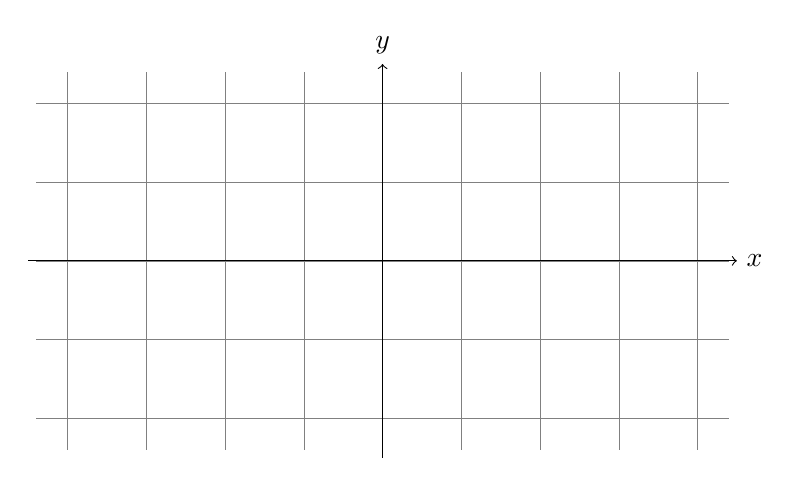
\begin{tikzpicture}
        \draw[help lines,step=1cm] (-4.4,-2.4) grid (4.4,2.4);
        \draw[->] (-4.5,0) -- (4.5,0) node[right] {$x$};
        \draw[->] (0,-2.5) -- (0,2.5) node[above] {$y$};
\end{tikzpicture}\]}
%   oz. za kompleksno ravnino \dodatek\[\begin{tikzpicture}
        \draw[help lines,step=1cm] (-4.4,-2.4) grid (4.4,2.4);
        \draw[->] (-4.5,0) -- (4.5,0) node[right] {$Re$};
        \draw[->] (0,-2.5) -- (0,2.5) node[above] {$Im$};
\end{tikzpicture}\]
%==========================================================================

\naloga[\tocke{4}]
  Načrtaj paralelogram s podatki $\alpha=60^\circ$, $a=6cm$ in $e=8cm$.



\naloga[\tocke{5}]
  Načrtaj trikotnik s podatki $\gamma =30^\circ$, $c=5cm$ in $t_c =4cm$.


  
\naloga[\tocke{5}]
  Glede na sliko izračunaj $x$ in $y$.
  \begin{figure}[H]
    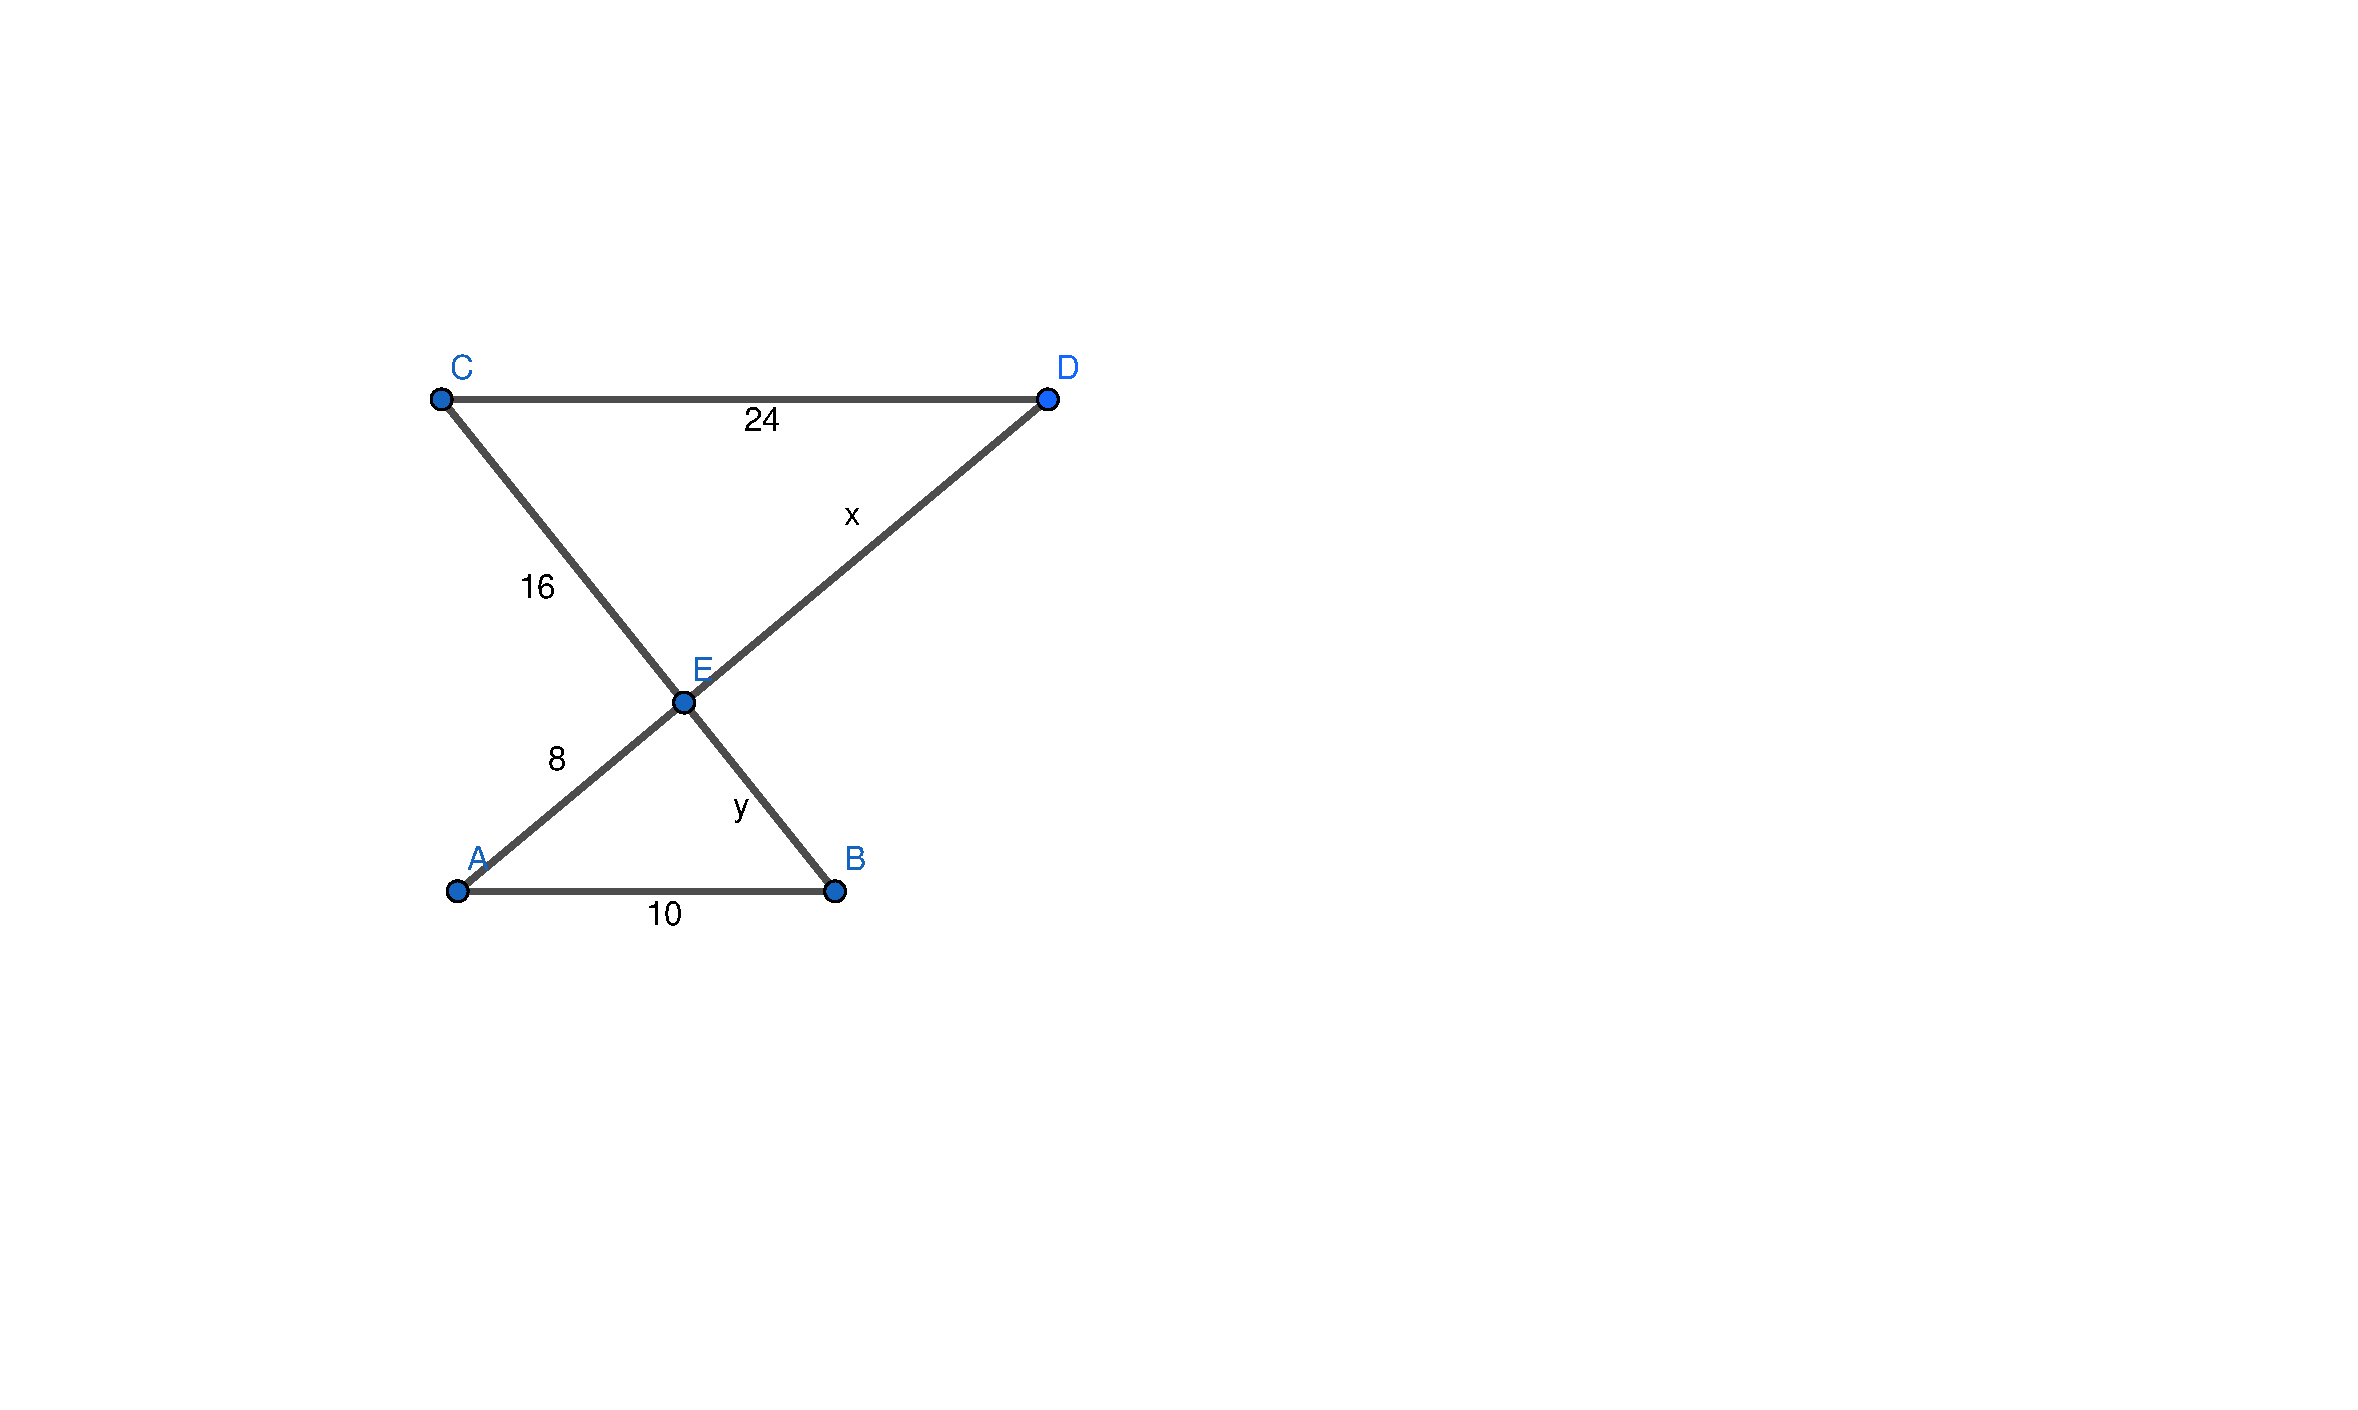
\includegraphics[width=1\textwidth]{geogebra-export.pdf}
    \centering
\end{figure}
  \prostor[2]

\naloga*[\tocke{4}]
  Število diagonal v nekem pravilnem večkotniku je za 25 večje od števila stranic. Izračunaj, koliko meri notranji kot tega večkotnika.
  \prostor[1.5]


\naloga[\tocke{4}]
  V pravokotnem trikotniku merita pravokotni projekciji katet na hipotenuzo $18cm$ in $32cm$. Izračunaj, koliko merijo stranice tega trikotnika in koliko meri višina.
  \prostor[1]

\naloga*[\tocke{3}]
  %Poenostavi $\left(1-\cos^2 x\right)(1+\cot^2 x)$.
  %Koliko stran od drevesa, visokega $35m$, se moramo postaviti, da ga vidimo pod kotom $30^\circ$?
  Natančno izračunaj, koliko je visok stolp, ki ga mravlja, ko se od stolpa oddalji za $20m$, vidi vrh stolpa pod kotom $30^\circ$.
  \prostor[1]





\end{document}